\documentclass[]{article}
\usepackage{lmodern}
\usepackage{amssymb,amsmath}
\usepackage{ifxetex,ifluatex}
\usepackage{fixltx2e} % provides \textsubscript
\ifnum 0\ifxetex 1\fi\ifluatex 1\fi=0 % if pdftex
  \usepackage[T1]{fontenc}
  \usepackage[utf8]{inputenc}
\else % if luatex or xelatex
  \ifxetex
    \usepackage{mathspec}
    \usepackage{xltxtra,xunicode}
  \else
    \usepackage{fontspec}
  \fi
  \defaultfontfeatures{Mapping=tex-text,Scale=MatchLowercase}
  \newcommand{\euro}{€}
\fi
% use upquote if available, for straight quotes in verbatim environments
\IfFileExists{upquote.sty}{\usepackage{upquote}}{}
% use microtype if available
\IfFileExists{microtype.sty}{%
\usepackage{microtype}
\UseMicrotypeSet[protrusion]{basicmath} % disable protrusion for tt fonts
}{}
\ifxetex
  \usepackage[setpagesize=false, % page size defined by xetex
              unicode=false, % unicode breaks when used with xetex
              xetex]{hyperref}
\else
  \usepackage[unicode=true]{hyperref}
\fi
\usepackage[usenames,dvipsnames]{color}
\hypersetup{breaklinks=true,
            bookmarks=true,
            pdfauthor={Leanne Lee},
            pdftitle={Stat 159 HW 2},
            colorlinks=true,
            citecolor=blue,
            urlcolor=blue,
            linkcolor=magenta,
            pdfborder={0 0 0}}
\urlstyle{same}  % don't use monospace font for urls
\usepackage{graphicx,grffile}
\makeatletter
\def\maxwidth{\ifdim\Gin@nat@width>\linewidth\linewidth\else\Gin@nat@width\fi}
\def\maxheight{\ifdim\Gin@nat@height>\textheight\textheight\else\Gin@nat@height\fi}
\makeatother
% Scale images if necessary, so that they will not overflow the page
% margins by default, and it is still possible to overwrite the defaults
% using explicit options in \includegraphics[width, height, ...]{}
\setkeys{Gin}{width=\maxwidth,height=\maxheight,keepaspectratio}
\setlength{\parindent}{0pt}
\setlength{\parskip}{6pt plus 2pt minus 1pt}
\setlength{\emergencystretch}{3em}  % prevent overfull lines
\providecommand{\tightlist}{%
  \setlength{\itemsep}{0pt}\setlength{\parskip}{0pt}}
\setcounter{secnumdepth}{0}

\title{Stat 159 HW 2}
\author{Leanne Lee}
\date{October 5, 2016}

% Redefines (sub)paragraphs to behave more like sections
\ifx\paragraph\undefined\else
\let\oldparagraph\paragraph
\renewcommand{\paragraph}[1]{\oldparagraph{#1}\mbox{}}
\fi
\ifx\subparagraph\undefined\else
\let\oldsubparagraph\subparagraph
\renewcommand{\subparagraph}[1]{\oldsubparagraph{#1}\mbox{}}
\fi

\begin{document}
\maketitle

\subsection{Abstract}\label{abstract}

This homework is to reproduce the analysis from Section 3.1 of Ch 3
Linear Regression from the book ``An Introduction to Statistical
Learning'' (by James et al). The homework will analyze the advertising
dataset with linear regression and summary statistics.

\subsection{Introduction}\label{introduction}

From the dataset advertising, I can reproduce the simple linear
regression with TV and sales. The simple linear regression can predict a
quantitative response Y based on predictor variable X. With the
modeling, we can tell if there is a relationship exists between TV
advertising and Sales. If there exists a positive relationship, the
marketing team can decide to increase Tv advertising budget to promote
their sales.

\subsection{Data}\label{data}

The dataset \emph{Advertising.csv} comes from
\_``http://www-bcf.usc.edu/\textasciitilde{}gareth/ISL/Advertising.csv\_.
It consists for TV, Radio, Newspaper and Sales columns. The structure of
the columns are stored in numeric vectors.

\subsection{Methodology}\label{methodology}

By using the simple linear regression, we can predict the future sales
based on the amount of TV advertising.\\
The simple linear regression equation is the following:

\begin{verbatim}
Y = A + Bx + e
\end{verbatim}

Y = Sales A = Intercept Bx = TV advertising e = error

In R command, we can fit a linear regression model by using the
\emph{lm()} command. The null hypothesis is there does not exist a
relationship between TV ad and sales. The alternative hypothesis is that
there exists a relationship between TV ad and sales. \#\#Results

\begin{verbatim}
load('./data/regression.RData')
library(xtable)
reg_table <- xtable(reg_summary)
reg_table
\end{verbatim}

\begin{figure}[htbp]
\centering
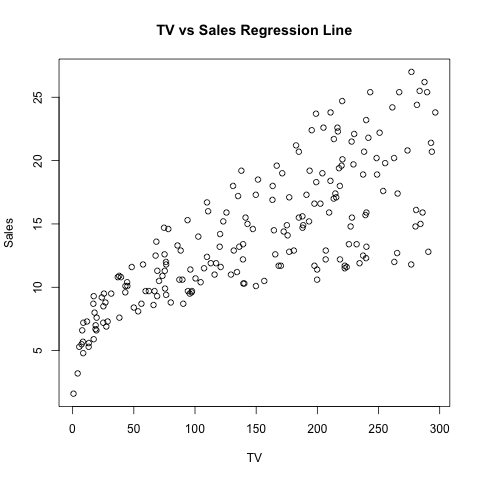
\includegraphics{./images/scatterplot-tv-sales.png}
\caption{TV ad vs sales linear regression scatter plot}
\end{figure}

\subsection{Conclusions}\label{conclusions}

This homework shows the relationship between TV advertising and sales.
There exists a positive correlation between the TV advertising and
sales. In the future, we can apply the same model to radio and
newspaper.

\end{document}
